\section{Mapserver}


\subsection{Cara Instalasi Mapserver}
\begin{enumerate}
\item
Download Mapserver atau disingkat MS4W di http://mapserver.org/download.html
\begin{figure}[ht]
	    \centerline{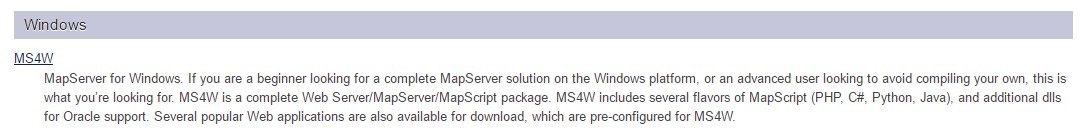
\includegraphics[width=0.50\textwidth]{figures/gambar1.JPG}}
	    \caption{Download MS4W}
		\label{gambar1}
		\end{figure}
\item
Setelah di download jalankan setupnya, disini saya menggunakan port 2000 karena port default 80 sudah dipakai oleh xampp
\begin{figure}[ht]
	    \centerline{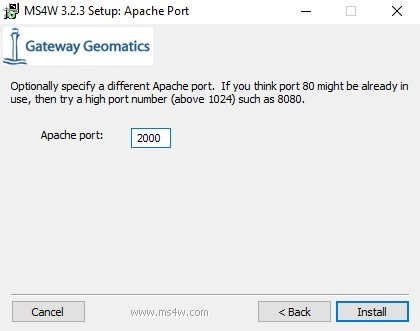
\includegraphics[width=0.50\textwidth]{figures/gambar2.JPG}}
	    \caption{Port 2000}
		\label{gambar2}
		\end{figure}
\item
Lalu tunggu instalasi sampai selesai
\begin{figure}[ht]
	    \centerline{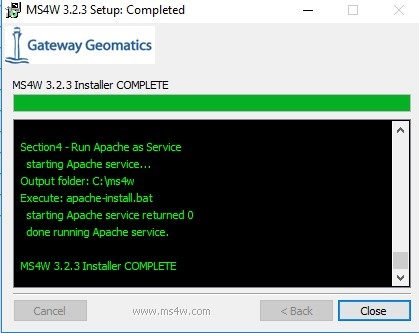
\includegraphics[width=0.50\textwidth]{figures/gambar3.JPG}}
	    \caption{Selesai}
		\label{gambar3}
		\end{figure}
\item
Setelah proses selesai silahkan buka browser favorit anda, kemudian ketikkan http://localhost:2000 di kotak isian URL.
\item
Jika anda melihat tampilan home MAPSERVER atau MS4W proses instalasi anda berhasil.
\begin{figure}[ht]
	    \centerline{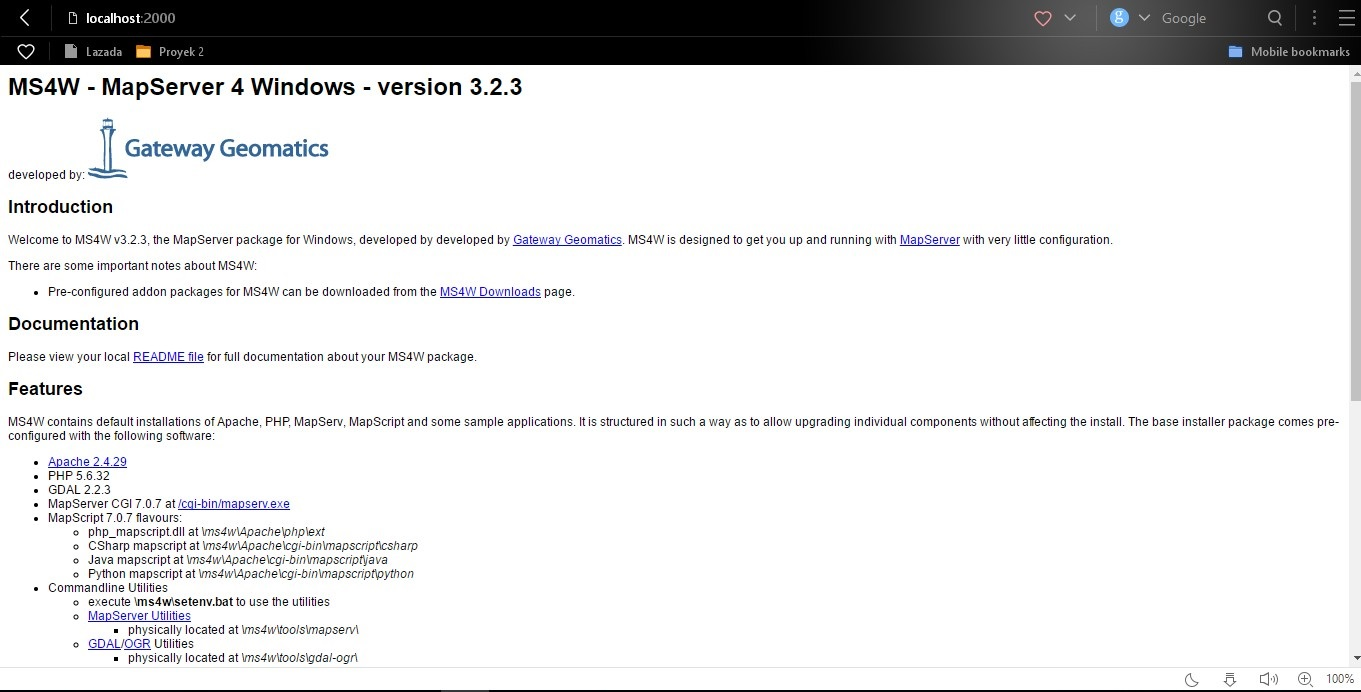
\includegraphics[width=0.50\textwidth]{figures/gambar4.JPG}}
	    \caption{Tampilan MS4W}
		\label{gambar4}
		\end{figure}
\end{enumerate}